\chapter{Cơ sở lý thuyết}
\section{Các cơ sở lý thuyết và công nghệ sử dụng}
\subsection{Reactjs}
\subsubsection{Khái niệm}
\indent ReactJS là một thư viện JavaScript phía người dùng (frontend) được sử dụng để xây dựng giao diện người dùng tương tác \footnote{https://fptcloud.com/reactjs/}.
\subsubsection{Ưu điểm của Reactjs}
\begin{itemize}
    \item \textbf{Tận dụng lại các thành phần có sẵn}

    \indent ReactJS hỗ trợ tích cực trong khởi tạo một website bởi lập trình viên sẽ không cần phải code nhiều như khi tạo trang web mà chỉ sử dụng JavaScript. Đồng thời, nó cung cấp một loạt các thành phần sẵn có mà bạn có thể sử dụng trong nhiều tình huống khác nhau.
    \item \textbf{Tích hợp được cho cả ứng dụng di động Mobile application}

    \indent Hầu hết chúng ta đã biết rằng ReactJS được sử dụng để phát triển các ứng dụng web, tuy nhiên, nó không chỉ giới hạn trong lĩnh vực đó. Nếu chúng ta muốn phát triển các ứng dụng di động, chúng ta có thể sử dụng React Native. Đây là một framework do Facebook phát triển, cho phép chúng ta dễ dàng "chia sẻ" các thành phần và tái sử dụng logic nghiệp vụ trong các ứng dụng của chúng ta.
    \item \textbf{Tối ưu để tăng cường khả năng tìm kiếm SEO}

    \indent Tối ưu hóa công cụ tìm kiếm (SEO) là một yếu tố quan trọng để đảm bảo trang web của chúng ta xuất hiện cao hơn trong kết quả tìm kiếm của Google. ReactJS là một thư viện JavaScript cơ bản. Công cụ tìm kiếm của Google có khả năng thu thập thông tin và lập chỉ mục mã JavaScript, tuy nhiên, nó cũng yêu cầu sự hỗ trợ từ các thư viện khác để làm điều này.
    \item \textbf{Dễ dàng sửa lỗi và gỡ rối Debug}

    \indent Facebook đã phát hành một tiện ích mở rộng Chrome để hỗ trợ việc gỡ lỗi trong quá trình phát triển ứng dụng. Điều này giúp tăng tốc quá trình phát hành sản phẩm cũng như quá trình viết mã của chúng ta.
\end{itemize}
\subsubsection{Nhược điểm của Reactjs}
\begin{itemize}
    \item Reactjs không phải là framework, cho nên chúng ta phải tự xây dựng dự án bằng thủ công.
    \item Tích hợp Reactjs vào các framework MVC truyền thống yêu cầu cần phải cấu hình lại.
    \item Poor Document: Đó là một nhược điểm khá phổ biến đối với các công nghệ cập nhật liên tục. Các công nghệ cập nhật và tăng tốc nhanh đến mức không có thời gian để tạo tài liệu phù hợp.
\end{itemize}
\subsection{Java Spring Boot}

\subsubsection{Khái niệm:} Spring Boot là một framework phát triển ứng dụng Java, dựa trên nền tảng Spring Framework. Nó được thiết kế để giảm bớt công việc cấu hình và cung cấp một cách tiếp cận linh hoạt và nhanh chóng để xây dựng các ứng dụng Java.\footnote{https://lotusacademy.edu.vn/blog/java-spring-boot-la-gi-java-spring-mvc-la-gi-spring-framework-la-gi-256}

\subsubsection{Ưu điểm:}
\begin{itemize}
    \item \textbf{Tự động cấu hình:} Spring Boot tự động cấu hình dựa trên các quy tắc mặc định và cung cấp một số cấu hình tùy chỉnh đơn giản.
    \item \textbf{Tiết kiệm thời gian:} Với Spring Boot, bạn không cần lo lắng về việc cấu hình chi tiết và tập trung vào việc phát triển chức năng của ứng dụng.
    \item \textbf{Tích hợp dễ dàng:} Spring Boot tích hợp tốt với các công nghệ và thư viện phổ biến khác, cho phép bạn dễ dàng tích hợp các thành phần khác như cơ sở dữ liệu, bảo mật, gửi email, vv.
    \item \textbf{Gói hóa ứng dụng:} Spring Boot cho phép bạn gói hóa ứng dụng thành file JAR hoặc WAR, giúp dễ dàng triển khai và chạy trên các môi trường khác nhau.
\end{itemize}

\subsubsection{Nhược điểm:}
\begin{itemize}
    \item \textbf{Phụ thuộc:} Spring Boot có thể tạo ra các ứng dụng có phụ thuộc tăng cao vào framework, điều này có thể làm cho ứng dụng phải dựa vào các phiên bản và cấu hình cụ thể của Spring Boot.
    \item \textbf{Tính linh hoạt:} Mặc dù Spring Boot giảm bớt công việc cấu hình, nhưng đôi khi nó có thể hạn chế tính linh hoạt so với việc cấu hình thủ công bằng XML hoặc Java.
    \item \textbf{Độ phức tạp:} Một số tính năng và cấu hình cao cấp của Spring Boot có thể trở nên phức tạp và khó hiểu đối với những người mới sử dụng.
\end{itemize}
\indent Tuy nhiên, ưu điểm của Spring Boot thường vượt trội hơn so với nhược điểm, vì nó giúp đơn giản hóa việc phát triển và triển khai ứng dụng Java.

\subsection{Nodejs}
\subsubsection{Khái niệm}
\indent Node.js là một môi trường chạy mã JavaScript phía máy chủ, dựa trên JavaScript Engine V8 của Google. Nó cho phép viết mã JavaScript để xây dựng ứng dụng máy chủ một cách hiệu quả. \footnote{https://nodejs.org/en/about}
\subsubsection{Ưu điểm của Node.js:}
\begin{itemize}
    \item Hiệu suất cao: Với JavaScript Engine V8 nhanh chóng, Node.js cho phép xử lý các yêu cầu đồng thời một cách hiệu quả và đạt được hiệu suất cao.
    \item Đơn luồng và không đồng bộ: Node.js sử dụng mô hình xử lý không đồng bộ (non-blocking) I/O, giúp xử lý nhiều yêu cầu cùng một lúc mà không tốn thêm tài nguyên.
    \item Quản lý gói dễ dàng: Node.js có npm (Node Package Manager), cung cấp một kho lưu trữ gói phong phú và dễ quản lý.
    \item Phát triển đồng nhất: Với Node.js, phát triển ứng dụng web và ứng dụng di động có thể được thực hiện bằng cùng một ngôn ngữ và công cụ, tạo sự đồng nhất.
\end{itemize}
\subsubsection{Nhược điểm của Node.js:}
\begin{itemize}
    \item Chưa phù hợp cho các tác vụ nặng: Do Node.js sử dụng mô hình đơn luồng, nó không phù hợp cho các tác vụ tính toán nặng hoặc xử lý dữ liệu lớn.
    \item Đòi hỏi khéo léo trong việc quản lý bộ nhớ: Node.js không tự động quản lý bộ nhớ, điều này yêu cầu phải làm việc thủ công để tránh rò rỉ bộ nhớ.
\end{itemize}
\subsection{Docker}
\subsubsection{Khái niệm:}
\indent Docker là một nền tảng mã nguồn mở giúp đóng gói các ứng dụng và các phụ thuộc của chúng vào những đơn vị gọi là containers. Containers cho phép triển khai một ứng dụng một cách đáng tin cậy và di động với sự độc lập về môi trường.\footnote{https://docs.docker.com/}
\subsubsection{Ưu điểm:}
\begin{itemize}
    \item Đóng gói và triển khai dễ dàng: Docker giúp đóng gói các ứng dụng và phụ thuộc vào một container có thể di chuyển được và triển khai một cách dễ dàng trên nhiều môi trường khác nhau.
    \item Tính nhất quán giữa môi trường phát triển và triển khai: Docker đảm bảo môi trường chạy ứng dụng trên máy chủ phát triển giống với môi trường chạy trên môi trường triển khai.
    \item Hiệu suất cao: Containers Docker nhẹ và nhanh chóng, giúp tối ưu hóa tài nguyên và cung cấp hiệu suất cao cho các ứng dụng.
\end{itemize}
\subsubsection{Nhược điểm:}
\begin{itemize}
    \item Tăng phức tạp: Đôi khi quản lý các container Docker và xử lý các phụ thuộc có thể trở nên phức tạp, đặc biệt là trong các môi trường lớn và phức tạp.
    \item Hiệu suất ảnh hưởng: Mặc dù Docker giúp tối ưu hóa hiệu suất, nhưng việc sử dụng container cũng có thể ảnh hưởng đến hiệu suất so với việc chạy ứng dụng trực tiếp trên máy chủ vật lý.
\end{itemize}

\subsection{Terraform}
\subsubsection{Khái niệm:}
\indent Terraform là một công cụ mã hóa cấu hình (Infrastructure as Code) được sử dụng để tự động hóa việc triển khai và quản lý cơ sở hạ tầng đám mây và hạ tầng điện toán.\footnote{https://www.alibabacloud.com/blog/terraform}
\subsubsection{Ưu điểm:}
\begin{itemize}
    \item Tự động hóa hạ tầng: 
    Terraform cho phép viết mã để mô tả và triển khai cơ sở hạ tầng một cách dễ dàng và nhất quán.
    \item Đa nền tảng: 
    Terraform hỗ trợ nhiều nhà cung cấp đám mây và nền tảng hạ tầng khác nhau như AWS, Azure, GCP, v.v., giúp quản lý và triển khai đồng nhất trên nhiều môi trường.
    \item Kiểm soát phiên bản: 
    Terraform quản lý các tài nguyên hạ tầng như mã nguồn, cho phép theo dõi và quản lý phiên bản tài nguyên trong quá trình phát triển và triển khai.
\end{itemize}
\subsubsection{Nhược điểm:}
\begin{itemize}
    \item Học và quản lý đòi hỏi thời gian: Terraform có độ dốc học đôi khi khá lớn, và việc quản lý mã cấu hình có thể đòi hỏi thời gian và kỹ năng.
    \item Giới hạn của các nhà cung cấp đám mây: Các nhà cung cấp đám mây có thể không hỗ trợ tất cả các tính năng của Terraform hoặc có giới hạn trong việc quản lý hạ tầng.
\end{itemize}
\subsection{Kubernetes}
\subsubsection{Khái niệm:}
\indent Kubernetes (thường được gọi là k8s) là một nền tảng mã nguồn mở để quản lý việc triển khai, tự động hóa và mở rộng ứng dụng container.\footnote{https://kubernetes.io/vi/docs/concepts/overview/what-is-kubernetes/}

\indent Các ứng dụng có sử dụng Kubernetes: Google, Netflix, Airbnb, Spotify, Grab, Zalando, Adidas...và nhiều hơn nữa. Kubernetes đã trở thành một công nghệ phổ biến và mạnh mẽ trong việc quản lý và triển khai ứng dụng quy mô lớn.
\subsubsection{Kiến trúc}
 \begin{figure}[H]
    \begin{center}
    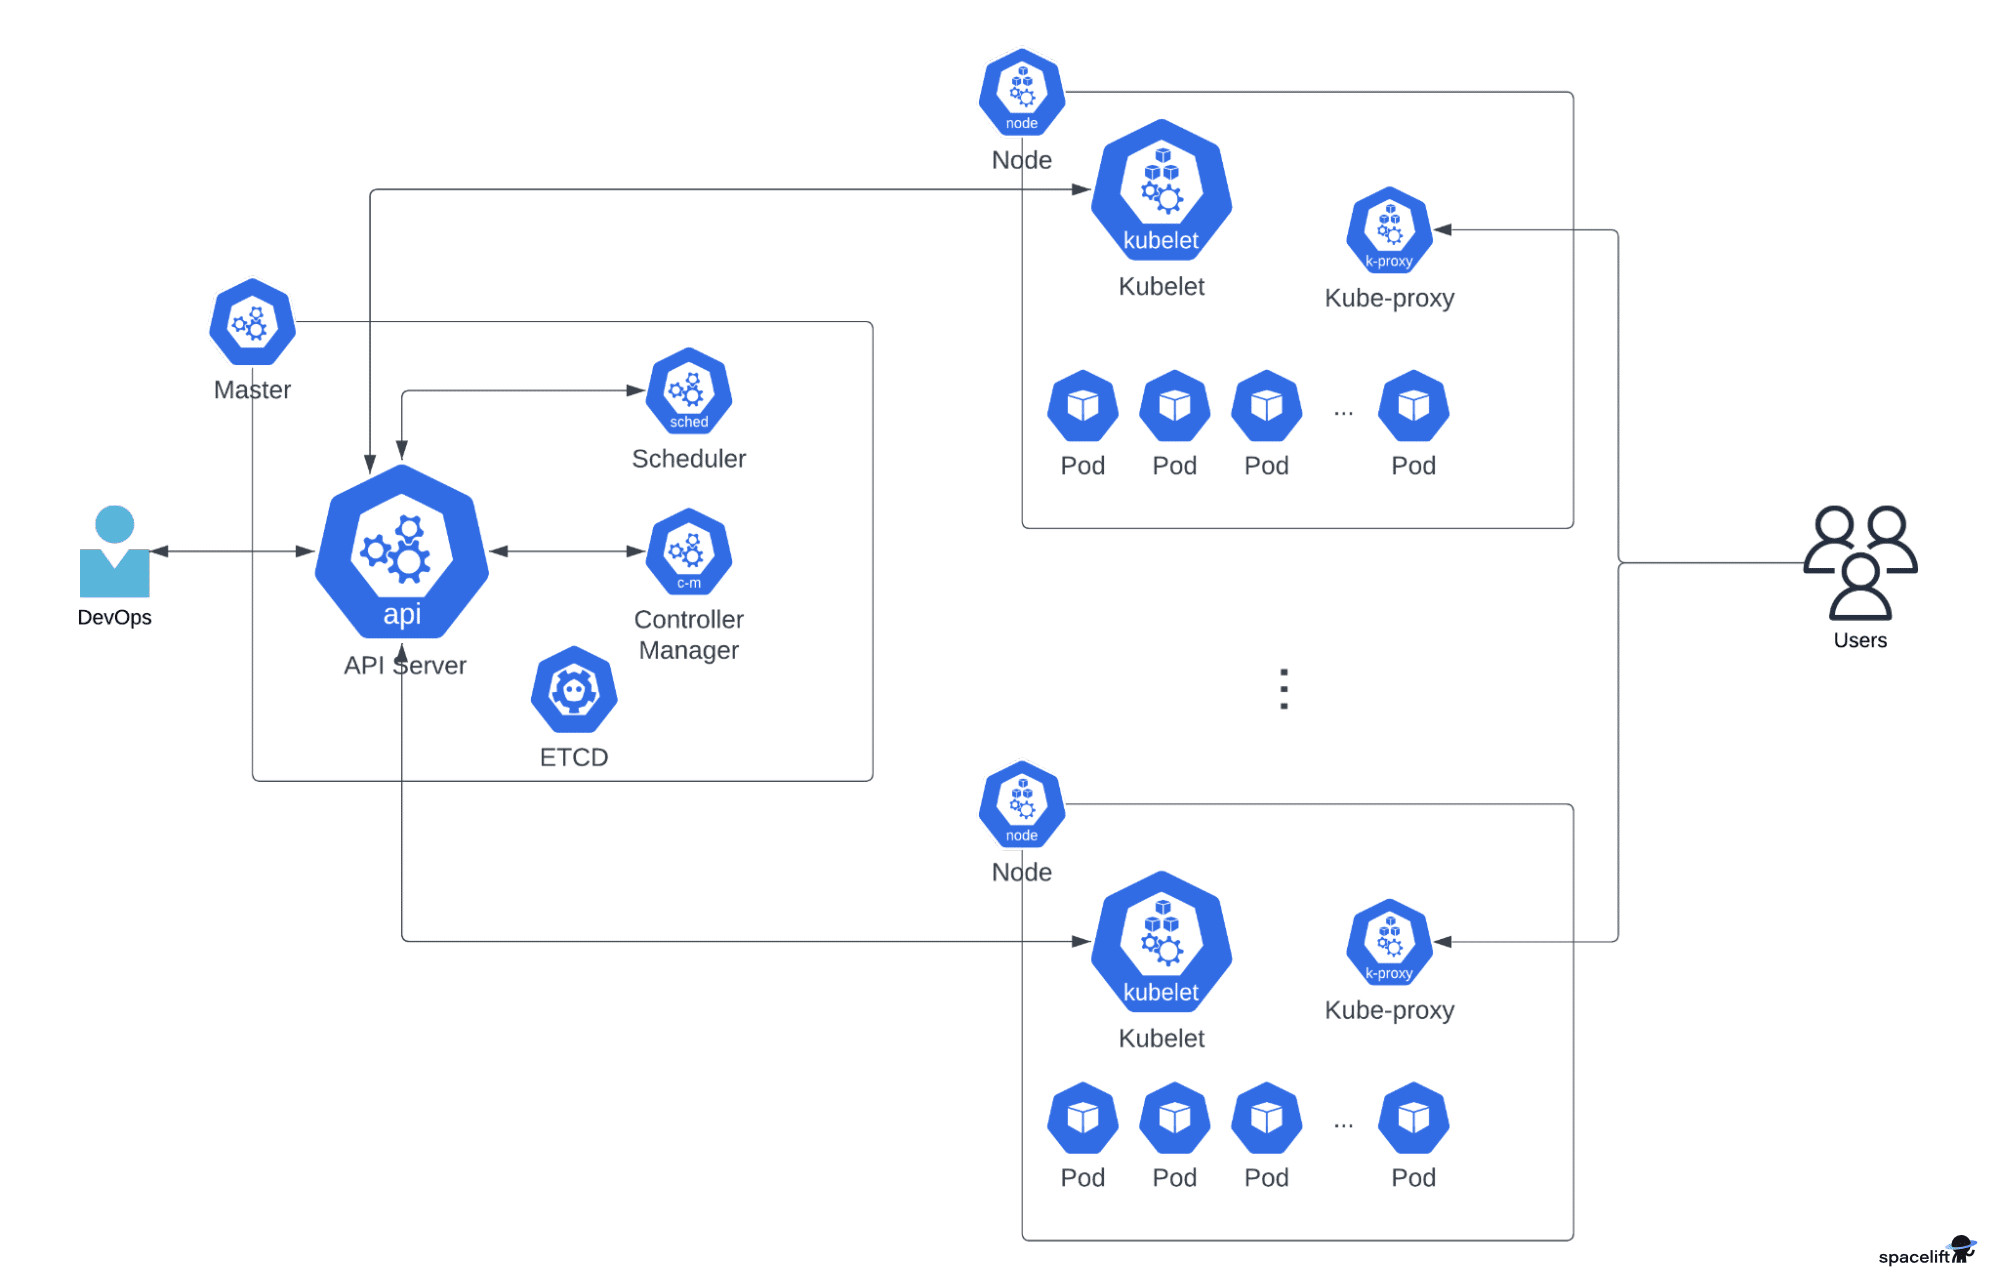
\includegraphics[scale = 0.22]{images/chap-2-images/kubernetes_architecture.jpg}
    \vspace*{7mm}
    \caption{Kubernetes Architecture }
    \end{center}
    \label{}
\end{figure}
\indent Kiến trúc của Kubernetes bao gồm:
\begin{itemize}
    \item Master Node: Quản lý, điều phối và giám sát toàn bộ hệ thống Kubernetes.
    \item Worker Node: Chứa các container và chịu trách nhiệm thực hiện các tác vụ đồng bộ từ Master Node.
    \item Pod: Nhóm các container chạy cùng nhau trên cùng một Worker Node, chia sẻ tài nguyên và mạng.
    \item Service: Một tập hợp các Pod có thể truy cập thành một đầu nối duy nhất từ bên ngoài.
    \item Volume: Cung cấp quản lý lưu trữ cho các container trong Pod.
\end{itemize}
\subsubsection{Cách thiết lập Kubernetes cho ứng dụng}
\begin{itemize}
    \item Định nghĩa và triển khai mô tả ứng dụng: Sử dụng các tệp cấu hình (ví dụ: YAML) để định nghĩa ứng dụng, bao gồm Pod, Service và các tài nguyên khác.
    \item Triển khai và quản lý: Gửi yêu cầu triển khai tới Master Node, sau đó Kubernetes sẽ triển khai các Pod và Service, quản lý vòng đời và giám sát.
    \item Tự động mở rộng và cân bằng tải: Kubernetes tự động mở rộng hoặc thu hẹp quy mô của các Pod để đáp ứng tải công việc và cân bằng tải giữa các Worker Node.
\end{itemize}
\subsubsection{Ưu điểm:}
\begin{itemize}
    \item Tự động hóa và quản lý quy mô: Kubernetes cho phép tự động mở rộng và thu hẹp quy mô các thành phần ứng dụng, như các microservice và cụm máy chủ. Điều này giúp tối ưu hóa hiệu suất và đáp ứng đối với lưu lượng truy cập thay đổi.

    \item Đảm bảo sẵn lòng và tin cậy: Kubernetes có khả năng phục hồi lỗi tự động và chuyển đổi dịch vụ giữa các phiên bản trên các nút khác nhau. Điều này giúp đảm bảo rằng ứng dụng luôn sẵn sàng và hoạt động một cách tin cậy.

    \item Quản lý tài nguyên hiệu quả: Kubernetes cung cấp các công cụ quản lý tài nguyên để phân bổ và giám sát tài nguyên phù hợp, bao gồm bộ nhớ, CPU, lưu trữ và mạng. Điều này giúp tối ưu hóa sử dụng tài nguyên và tăng hiệu suất hệ thống.

\end{itemize}
\subsubsection{Nhược điểm:}
\begin{itemize}
    \item Đòi hỏi kiến thức phức tạp: Kubernetes có độ dốc học và quản lý phức tạp, đòi hỏi kiến thức về hạ tầng và kỹ năng quản lý container.
    \item Tài nguyên tốn kém: Kubernetes yêu cầu sự sẵn có của một cụm máy chủ và tài nguyên đáng kể để triển khai và vận hành.
\end{itemize}
\subsection{Redis Cache}
\subsubsection{Khái niệm:}
\indent Redis Cache là một cơ sở dữ liệu key-value (khóa-giá trị) phân tán, được sử dụng để lưu trữ dữ liệu tạm thời trong bộ nhớ. \footnote{https://kdata.vn/cam-nang/redis-la-gi-hieu-ro-ve-he-thong-co-so-du-lieu-trong-bo-nho}
\subsubsection{Ưu điểm:}
\begin{itemize}
    \item Tốc độ và hiệu suất cao: Redis Cache lưu trữ dữ liệu trong bộ nhớ và cho phép truy cập cực kỳ nhanh chóng, đáp ứng yêu cầu với hiệu suất cao.
    \item Đa dạng tính năng: Redis cung cấp nhiều tính năng như caching, xử lý hàng đợi, pub/sub messaging và phân tích dữ liệu, giúp tối ưu hóa các tác vụ dựa trên dữ liệu.
\end{itemize}
\subsubsection{Nhược điểm:}
\begin{itemize}
    \item Giới hạn bộ nhớ: Redis Cache yêu cầu bộ nhớ đủ lớn để lưu trữ dữ liệu. Nếu dữ liệu vượt quá dung lượng bộ nhớ, có thể gặp sự cố và ảnh hưởng đến hiệu suất.
    \item Khả năng mất dữ liệu: Redis Cache mặc định không cung cấp cơ chế đồng bộ hoá dữ liệu, điều này đồng nghĩa rằng có thể mất dữ liệu khi xảy ra sự cố.
\end{itemize}
\subsection{PostgreSQL}
\subsubsection{Khái niệm:}
\indent PostgreSQL (viết tắt là Postgres) là một hệ quản trị cơ sở dữ liệu quan hệ mã nguồn mở, được đánh giá là ổn định, mạnh mẽ và có tính mở rộng.
\subsubsection{Ưu điểm:}
\begin{itemize}
    \item Độ tin cậy cao: PostgreSQL được thiết kế để đảm bảo tính toàn vẹn và độ tin cậy của dữ liệu, bao gồm các tính năng như ACID và khả năng khôi phục dữ liệu.
    \item Tính mở rộng và phân vùng: PostgreSQL hỗ trợ phân vùng dữ liệu và khả năng mở rộng sẵn sàng, cho phép mở rộng cơ sở dữ liệu để xử lý lượng dữ liệu lớn và tải cao.
    \item Đa dạng tính năng: PostgreSQL cung cấp nhiều tính năng tiên tiến bao gồm trình tự, trigger, tìm kiếm văn bản và hình ảnh, và hỗ trợ các loại dữ liệu phong phú.
\end{itemize}
\subsubsection{Nhược điểm:}
\begin{itemize}
    \item Có thể cảm thấy phức tạp đối với các dự án nhỏ.
\end{itemize}
\subsection{EKS}
\subsubsection{Khái niệm:}
\indent EKS (Elastic Kubernetes Service) là một dịch vụ quản lý Kubernetes do Amazon Web Services (AWS) cung cấp.
\subsubsection{Ưu điểm:}
\begin{itemize}
    \item Dễ dàng triển khai, quản lý và mở rộng các ứng dụng chạy trên Kubernetes.
    \item Tích hợp tốt với dịch vụ AWS khác.
    \item Hỗ trợ cho môi trường đám mây tiêu chuẩn và quy mô lớn.
\end{itemize}
\subsubsection{Nhược điểm:}
\begin{itemize}
    \item Phí sử dụng có thể cao, đặc biệt trong trường hợp triển khai lớn.
    \item Đòi hỏi kiến thức về quản lý và triển khai hệ thống phức tạp hơn so với các giải pháp khác.
\end{itemize}
\subsection{AKS}
\subsubsection{Khái niệm:}
\indent AKS (Azure Kubernetes Service) là một dịch vụ quản lý Kubernetes.

\subsubsection{Ưu điểm:}
\begin{itemize}
    \item Dễ dàng triển khai, quản lý và mở rộng các ứng dụng chạy trên Kubernetes.
    \item Tích hợp tốt với dịch vụ Azure và công cụ phát triển của Microsoft.
    \item Cung cấp tính năng bảo mật và giám sát mạnh mẽ.
\end{itemize}
\subsubsection{Nhược điểm:}
\begin{itemize}
    \item Phí sử dụng có thể cao, đặc biệt trong trường hợp triển khai lớn.
    \item Yêu cầu sử dụng môi trường và công cụ phát triển Azure.
\end{itemize}
\subsection{RabbitMQ}
\subsubsection{Khái niệm:}
\indent RabbitMQ là một hệ thống message broker mã nguồn mở, dựa trên giao thức AMQP (Advanced Message Queuing Protocol).
 \begin{figure}[H]
    \begin{center}
    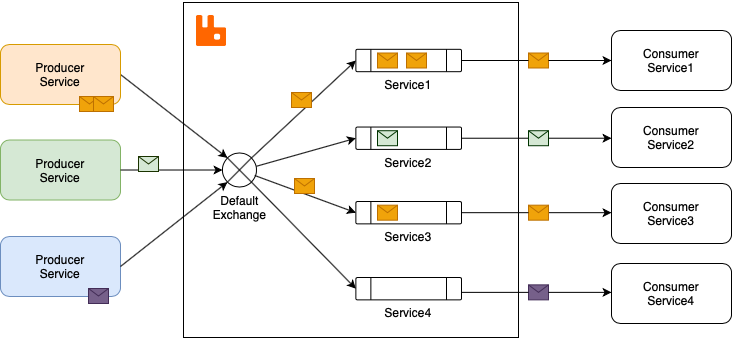
\includegraphics[scale = 0.5]{images/chap-2-images/rabbitMQ.png}
    \vspace*{7mm}
    \caption{RabbitMQ Architecture}
    \end{center}
    \label{}
\end{figure}
\subsubsection{Kiến trúc của RabbitMQ}
\begin{itemize}
    \item Producer:

Là thành phần tạo ra và gửi các thông điệp (message).
Message được gửi đến một exchange.
    \item Exchange:

Nhận thông điệp từ nhà sản xuất và định tuyến chúng đến hàng đợi (queue) thích hợp.
Có các loại định tuyến khác nhau như direct, topic, fanout, và headers, cho phép định tuyến dựa trên các tiêu chí khác nhau.
    \item Queue (Hàng đợi):

Là nơi lưu trữ các thông điệp đến từ sàn giao dịch cho đến khi chúng được xử lý bởi một tiêu thụ (consumer).
Các hàng đợi có thể được chia sẻ giữa nhiều tiêu thụ hoặc có thể chỉ được sử dụng bởi một tiêu thụ cụ thể.
    \item Binding (Ràng buộc):

Liên kết giữa một exchange và một queue, xác định cách thông điệp nên được định tuyến từ exchange đến queue.
Ràng buộc này được thiết lập thông qua các quy tắc định tuyến (routing key).
    \item Consumer:

Là thành phần đọc và xử lý các thông điệp từ hàng đợi.
Có thể có nhiều tiêu thụ cùng một lúc đọc từ cùng một hàng đợi.
    \item Virtual Host:

Là một không gian làm việc ảo trong RabbitMQ, giúp tách biệt và cô lập các ứng dụng và người dùng khác nhau.
Mỗi Virtual Host có thể có các exchange, queue, và quyền riêng biệt.
    \item Broker:

Là nền tảng hoạt động của RabbitMQ.
Nhận thông điệp từ nhà sản xuất, định tuyến chúng đến hàng đợi thông qua sàn giao dịch và chuyển giao chúng đến các tiêu thụ.
    \item Connection:

Là một kết nối mạng giữa ứng dụng và RabbitMQ Broker.
Mỗi ứng dụng có thể có nhiều kết nối.
\end{itemize}

\subsubsection{Ưu điểm:}
\begin{itemize}
    \item Hỗ trợ đa ngôn ngữ và dễ dàng tích hợp với các ứng dụng phổ biến.
    \item Cung cấp tính năng đám mây phân tán, đảm bảo bất đồng bộ và xử lý hàng đợi.
    \item Tích hợp tốt với các công nghệ và framework khác như Spring, .NET, Node.js, etc.
\end{itemize}
\subsubsection{Nhược điểm:}
\begin{itemize}
    \item Cấu hình phức tạp và yêu cầu kiến thức về hệ thống phân tán.
    \item Hiệu suất có thể bị ảnh hưởng đối với tải công việc rất cao.
\end{itemize}

\section{Case study}
\subsection{Ứng dụng kiến trúc microservice với Azure Kubernetes Service}
\begin{figure}[h]
    \centering
    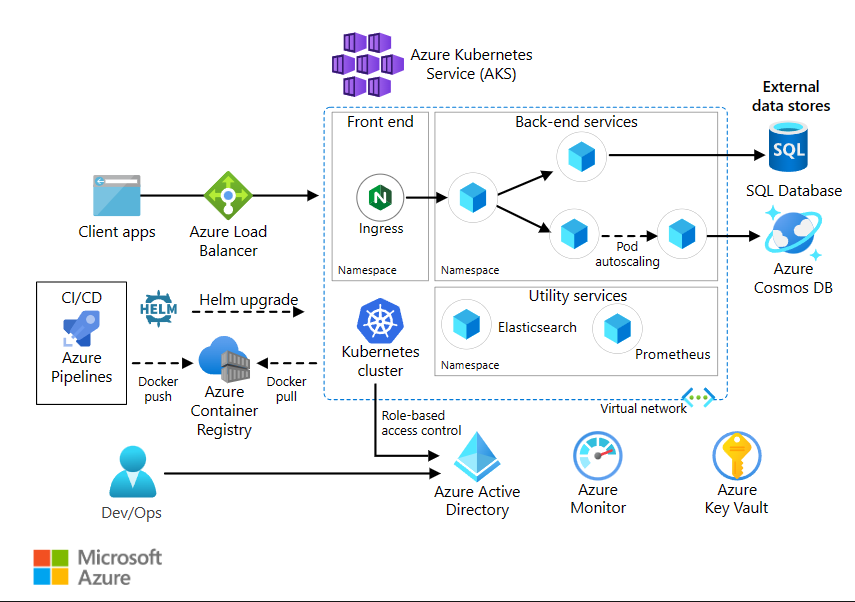
\includegraphics[scale=0.8]{images/hieu/chap-2/aks-architecture.png}
    \caption{AKS Architecture}
\end{figure}
\subsubsection{Các thành phần của kiến trúc}
\begin{itemize}
    \item \textbf{Azure Kubernetes Service (AKS)}: Là một dịch vụ quản lý Kubernetes do Microsoft cung cấp.Azure quản lý dịch vụ API Kubernetes và bạn chỉ cần quản lý các nút tác nhân (agent node).
    \item \textbf{Virtual Network}: Theo mặc định, AKS tạo một mạng ảo trong đó các nút tác nhân được kết nối. Trước tiên, bạn có thể tạo mạng ảo cho các tình huống nâng cao hơn, cho phép bạn kiểm soát những thứ như cấu hình mạng con.
    \item \textbf{Ingress}:Ingress hiển thị các tuyến HTTPs tới các dịch vụ bên trong cluster.
    \item \textbf{Azure Load Balancer}:sau khi tạo AKS cluster, cluster đã sẵn sàng sử dụng bộ cân bằng tải. Khi dịch vụ NGINX được triển khai, bộ cân bằng tải sẽ được cấu hình bằng một IP công cộng mới phía trước bộ điều khiển xâm nhập (ingress controller). Bằng cách này, bộ cân bằng tải định tuyến lưu lượng truy cập internet đến ingress.
    \item \textbf{Exteral Data Store}: Các microservice thường không có trạng thái (stateless) và trạng thái ghi vào các kho dữ liệu bên ngoài, chẳng hạn như Cơ sở dữ liệu Azure SQL hoặc Azure Cosmos DB.
    \item \textbf{Microsoft ID Entra}: AKS sử dụng Microsoft Entra ID để tạo và quản lý các tài nguyên Azure khác như bộ cân bằng tải Azure. Microsoft Entra ID cũng được khuyến nghị để xác thực người dùng trong các ứng dụng khách.
    \item \textbf{Azure Container Registry}: Azure Container Registry là một kho lưu trữ riêng tư cho các hình ảnh Docker. Nó được sử dụng để lưu trữ các hình ảnh Docker được sử dụng để triển khai các dịch vụ trong AKS cluster.
    \item \textbf{Azure Pipeline}: Azure Pipeline là một dịch vụ liên tục tích hợp và triển khai (CI/CD) được sử dụng để triển khai các dịch vụ trong AKS cluster.. Azure Pipelines là một phần của Dịch vụ Azure DevOps và chạy các bản dựng, thử nghiệm và triển khai tự động.
    \item \textbf{Helm}: Helm là một công cụ quản lý gói cho Kubernetes. Nó cho phép bạn định nghĩa, cài đặt và cập nhật các ứng dụng Kubernetes. Helm Charts là các gói Helm. Helm Charts được sử dụng để triển khai các ứng dụng trong AKS cluster.
    \item \textbf{Azure Monitor}: Azure Monitor là một dịch vụ giám sát đám mây. Nó cho phép bạn thu thập và phân tích dữ liệu từ nhiều nguồn khác nhau, bao gồm các dịch vụ Azure và các ứng dụng trên nhiều nền tảng. Azure Monitor được sử dụng để giám sát các dịch vụ trong AKS cluster.
\end{itemize}
\subsubsection{Một số cân nhắc}
\begin{itemize}
    \item \textbf{Design}:Kiến trúc tham chiếu này tập trung vào kiến trúc microservice, mặc dù nhiều phương pháp được đề xuất áp dụng cho các khối lượng công việc khác chạy trên AKS.
    \item \textbf{Microservice}:Microservice là một đơn vị mã có thể triển khai độc lập. Các microservice thường giao tiếp thông qua các API được xác định rõ ràng . Dịch vụ phải luôn có thể truy cập được ngay cả khi pod di chuyển xung quanh. Đối tượng Dịch vụ Kubernetes là một cách tự nhiên để mô hình hóa các dịch vụ vi mô trong Kubernetes.
    \item \textbf{API Gateway}:API gateway nằm giữa các máy khách bên ngoài và microservice. Nó hoạt động như một proxy ngược, định tuyến các yêu cầu từ máy khách đến microservice.
    \item \textbf{Data storage}:Trong kiến trúc microservice, các dịch vụ không nên chia sẻ giải pháp lưu trữ dữ liệu. Mỗi dịch vụ nên quản lý tập dữ liệu riêng của mình để tránh sự phụ thuộc ẩn giữa các dịch vụ.
Tránh lưu trữ dữ liệu liên tục trong bộ lưu trữ cluster cục bộ vì điều đó liên kết dữ liệu với node. Thay vào đó, hãy sử dụng dịch vụ bên ngoài như Cơ sở dữ liệu Azure SQL hoặc Azure Cosmos DB. Nếu bạn cần lưu trữ dữ liệu tạm thời, hãy sử dụng Redis Cache.
    \item \textbf{Namespace}:Namespace tổ chức các dịch vụ trong cluster, ngăn ngừa xung đột tên, áp dụng ràng buộc tài nguyên và chính sách bảo mật ở cấp độ namespace, và tổ chức microservice thành các ngữ cảnh được giới hạn thông qua việc tạo namespace cho từng ngữ cảnh. Đồng thời, việc đặt các dịch vụ tiện ích như Elasticsearch, Prometheus hoặc Tiller vào các namespace riêng biệt cũng được khuyến khích.
    \item \textbf{Health Probes}:Health probes là các yêu cầu HTTP được gửi đến các dịch vụ để xác định trạng thái của chúng. Nếu một dịch vụ không phản hồi, Kubernetes sẽ xóa pod và tạo lại nó. Điều này đảm bảo rằng các dịch vụ luôn sẵn sàng để phục vụ yêu cầu.
    \newline
    Kubernetes xác định hai loại thăm dò sức khỏe mà pod có thể hiển thị:
        \begin{itemize}
            \item Thăm dò sẵn sàng:Thăm dò sẵn sàng xác định khi nào pod đã sẵn sàng để phục vụ yêu cầu.  
            \item Thăm dò sự sống:Thăm dò sự sống xác định khi nào pod cần được khởi động lại. Nếu thăm dò sự sống thất bại, pod sẽ bị xóa và tạo lại.
        \end{itemize}
    Một số cân nhắc khi thiết kế health probes:
        \begin{itemize}
            \item Nếu mã của bạn có thời gian khởi động dài, có nguy cơ do trình thăm dò mức độ hoạt động sẽ báo cáo lỗi trước khi quá trình khởi động hoàn tất. Để giải quyết vấn đề này, hãy sử dụng cài đặt initialDelaySeconds để trì hoãn việc khởi động đầu dò.
            \item Việc thăm dò độ sống sẽ không giúp ích gì trừ khi việc khởi động lại pod có khả năng khôi phục nó về trạng thái khỏe mạnh. Bạn có thể sử dụng công cụ thăm dò mức độ hoạt động để giảm thiểu tình trạng rò rỉ bộ nhớ hoặc bế tắc không mong muốn, nhưng việc khởi động lại pod sẽ lại bị lỗi ngay lập tức sẽ chẳng ích gì.
            \item Đôi khi các thăm dò sẵn sàng được sử dụng để kiểm tra các dịch vụ phụ thuộc. 
            Ví dụ: nếu một pod phụ thuộc vào cơ sở dữ liệu thì đầu dò có thể kiểm tra kết nối cơ sở dữ liệu. 
            Tuy nhiên, cách tiếp cận này có thể tạo ra những vấn đề không mong muốn. 
            Một dịch vụ bên ngoài có thể tạm thời không khả dụng vì một số lý do. 
            Điều đó sẽ khiến cho việc thăm dò mức độ sẵn sàng không thành công đối với tất cả các pod trong dịch vụ của bạn, khiến tất cả các pod đó bị xóa khỏi cân bằng tải và do đó tạo ra lỗi xếp tầng ở thượng nguồn. 
            Cách tiếp cận tốt hơn là triển khai xử lý thử lại trong dịch vụ của bạn để dịch vụ của bạn có thể khôi phục chính xác sau các lỗi nhất thời.
        \end{itemize}
    \item \textbf{Resource constrain}: Tranh chấp tài nguyên có thể ảnh hưởng đến tính sẵn có của dịch vụ. Xác định các giới hạn tài nguyên cho các container để một container không thể áp đảo các tài nguyên của cluster (bộ nhớ và CPU).
    Sử dụng hạn ngạch tài nguyên để giới hạn tài nguyên được phép cho một namespace. 
    \item \textbf{Service object - SO}: Đôi tượng dịch vụ Kubernetes cung cấp một tập hợp các khả năng phù hợp với yêu cầu của microservice về khả năng khám phá dịch vụ:
        \begin{itemize}
            \item Địa chị IP: SO cung cấp một địa chỉ IP nội bộ tĩnh cho một pod (ReplicaSet) để các dịch vụ có thể truy cập tại địa chỉ này.
            \item Cân bằng tải (Load Balancer): Lưu lượng gửi đến địa chỉ IP của dịch vụ được cân bằng tải cho cácp pod.
            \item Khám phá dịch vụ (Service Recovery): SO cung cấp một tên miền DNS cho một dịch vụ, cổng API có thể gọi dịch vụ bằng tên miền này này. Các mục DNS được sắp xếp theo namespace.
        \end{itemize}
        \begin{figure}[h]
            \centering
            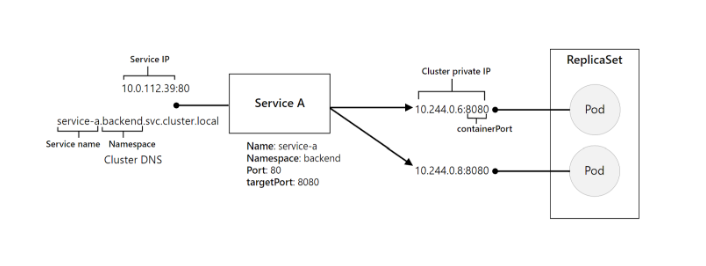
\includegraphics[scale=1]{images/hieu/chap-2/service-object-diagram.png}
            \caption{Sơ đồ mối quan hệ giữa các đối tượng dịch vụ và pod}  
        \end{figure}
    \item \textbf{Ingress}: Bộ điều khiển ingress (Ingress Controller) và ingress có thể phối hợp hoạt động để cung cấp các tính năng sau:
        \begin{itemize}
            \item Định tuyến các yêu cầu của khách hàng, định tuyến này cung cấp một điểm cuối duy nhất cho khách hàng và tách khách hàng khỏi các dịch vụ.
            \item Tổng hợp nhiều yêu cầu thành một yêu cầu duy nhất.
            \item Giảm tải chức năng như chấm dứt SSL, xác thực, hạn chế IP hoặc giới hạn tốc độ máy khách. 
        \end{itemize}
    \item \textbf{Mã hoá TLS/SSL}: Mã hoá TLS/SSL là một phương pháp mã hoá dữ liệu để bảo mật các kết nối giữa các máy khách và máy chủ.
\end{itemize}
\subsubsection{Security}
\begin{itemize}
    \item \textbf{Role-based Access Control}
    \newline
    Kubernetes và Azure đều có cơ chế kiểm soát truy cập dựa trên vai trò (RBAC):
    \begin{itemize}
        \item Azure RBAC kiểm soát quyền truy cập vào tài nguyên trong Azure, bao gồm khả năng tạo tài nguyên mới. Quyền có thể được chỉ định cho người dùng.
        \item Kubernetes RPAC kiểm soát các quyền đối với API Kubernetes. Để gán quyền Kubernetes cho người dùng, tạo vai trò và ràng buộc vai trò với người dùng.
    \end{itemize}
    AKS tích hợp hai chơ chế RBAC này, khi tạo một cụm AKS, bạn có thể đặt cấu hình cụm đó để sử dụng Microsoft Entra ID để xác thực người dùng. Người dùng Microsoft Entra ID cần được quản trị viên cụm tạo RoleBindings để cấp quyền truy cập cho người dùng hoặc nhóm người dùng.
    \item \textbf{Secrets management and application credentials}
    \newline
    Các ứng dụng và dịch vụ thường cần thông tin xác thực cho phép chúng kết nối với các dịch vụ bên ngoài như Bộ lưu trữ Azure hoặc Cơ sở dữ liệu SQL. Thách thức là giữ những thông tin xác thực này an toàn và không rò rỉ chúng.
    Dưới đây là một số tuỳ chọn để lưu trữ bí mật một cách an toàn:
        \begin{itemize}
            \item Azure Key Vault: Azure Key Vault là một dịch vụ quản lý khóa, bí mật và chứng chỉ. Nó cung cấp một nơi để lưu trữ các bí mật và khóa truy cập vào các dịch vụ bên ngoài. Các ứng dụng có thể truy cập Key Vault để lấy thông tin xác thực.
            \item Kubernetes Secrets: Kubernetes Secrets là một đối tượng Kubernetes được sử dụng để lưu trữ các bí mật. Các bí mật được lưu trữ dưới dạng cặp khóa-giá trị và có thể được sử dụng bởi các pod trong cụm.
            \item HashiCorp Vault: HashiCorp Vault là một dịch vụ quản lý khóa, bí mật và chứng chỉ mã nguồn mở. Nó cung cấp một nơi để lưu trữ các bí mật và khóa truy cập vào các dịch vụ bên ngoài. Các ứng dụng có thể truy cập Vault để lấy thông tin xác thực.
        \end{itemize}
    Việc sử dụng HashiCorp Vault hoặc Azure Key Vault là một giải pháp tốt hơn so với Kubernetes Secrets có thể mang lại mốt số lợi ích:
        \begin{itemize}
            \item Kiểm soát tập trung các bí mật
            \item Đảm bảo ràng tất cả các bí mật được mã hoá ở phần còn lại.
            \item Quản lý khoá tập trung.
            \item Kiểm soát truy cập bị mật.
            \item Kiểm toán.
        \end{itemize}
    \item \textbf{Container và Orchestrator security}
    Đây là những phương pháp được khuyến nghị để bảo vệ pods và container của bạn:
        \begin{itemize}
            \item Giám sát mối đe doạ (thread monitoring) bằng cách sử dụng Microsoft Defender cho Containers.
            \item Giám sát lỗ hổng (Vulnerabilities monitoring) bằng cách sử dụng Microsoft Defender dành cho đám mây hoặc giải pháp bên thứ ba có sẵn thông qua Azure Marketplace.
            \item Tự động vá hình ảnh bằng tác vụ ACR, một tính năng của Azure Register. 
            \item Lưu trữ image trong Azure Container Registry, một private registry đáng tin cậy. Sử dụng webhook xác thực tiếp nhận trong Kubernetes để đảm bảo rằng các nhóm chỉ có thể lấy hình ảnh từ cơ quan đăng ký đáng tin cậy.
        \end{itemize}
      
\end{itemize}
\newpage
\subsection {Ứng dụng AKS cho kiến trúc microservice nâng cao}
\begin{figure}[h]
    \centering
    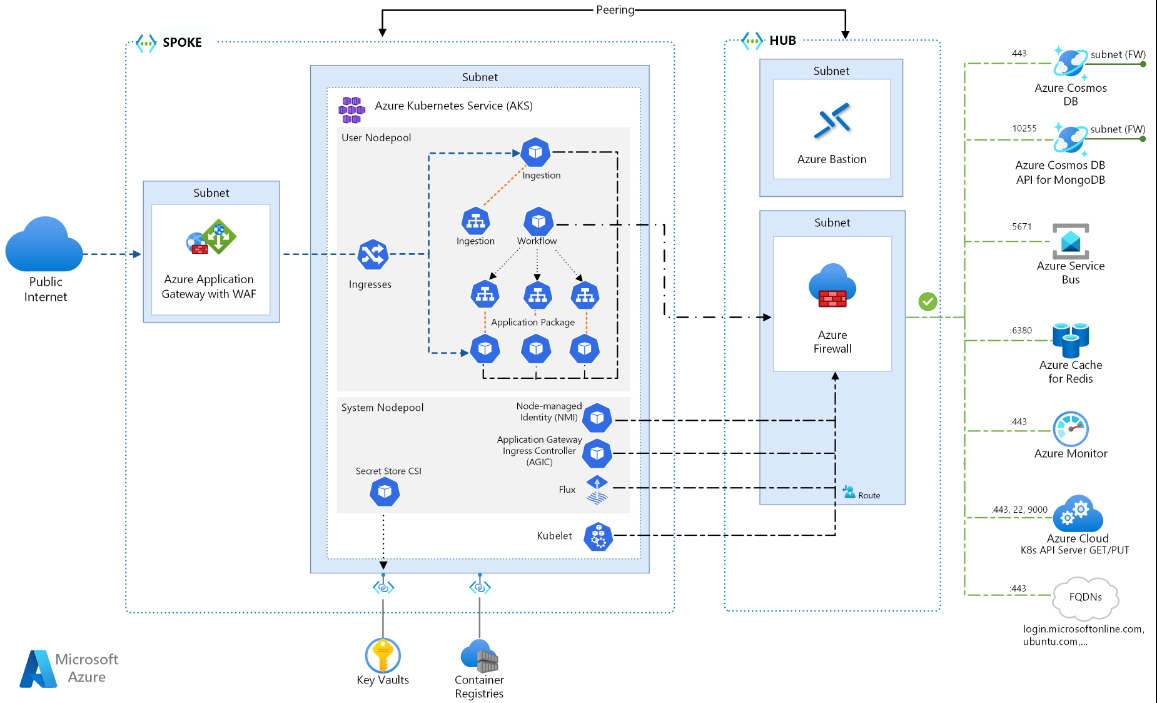
\includegraphics[scale=0.6]{images/hieu/chap-2/aks-architecture-advance.png}
    \caption{AKS Architecture Advance}
\end{figure}
\subsubsection{Workflow}
Luồng yêu cầu này triển khai các design pattern trên cloud Publisher-Subscriber, Competing Consumers, và Gateway Routing. Luồng tin nhắn diễn ra như sau:
    \begin{itemize}
        \item Một yêu cầu HTTPS được gửi để lên lịch nhận hàng bằng máy bay không người lái. Các yêu cầu chuyển qua Cổng ứng dụng Azure vào ứng dụng web nhập, ứng dụng này chạy dưới dạng vi dịch vụ trong cụm trong AKS.
        \item Ứng dụng web truyền dẫn sẽ tạo một thông báo và gửi nó đến hàng đợi thông báo Service Bus.
        \item Hệ thống phụ trợ chỉ định một máy bay không người lái và thông báo cho người dùng. Quy trình làm việc:
            \begin{itemize}
                \item Sử dụng thông tin tin nhắn từ hàng đợi tin nhắn Service Bus.
                \item Gửi yêu cầu HTTPS tới vi dịch vụ Phân phối để chuyển dữ liệu tới Bộ nhớ đệm Azure để lưu trữ dữ liệu ngoài của Redis.
                \item Gửi yêu cầu HTTPS tới microservice Drone Scheduler. 
                \item Gửi yêu cầu HTTPS tới vi dịch vụ Package, chuyển dữ liệu tới bộ lưu trữ dữ liệu bên ngoài MongoDB.
            \end{itemize} 
        \item Yêu cầu HTTPS GET được sử dụng để trả về trạng thái gửi. Yêu cầu này đi qua Cổng ứng dụng vào vi dịch vụ phân phối (Delivery Microservice).
        \item Vi dịch vụ phân phối đọc dữ liệu từ Azure Cache cho Redis.     
    \end{itemize}
\subsubsection{Các thành phần của kiến trúc}
Kiến trúc này sử dụng các thành phần Azure sau:
\begin{itemize}
    \item \textbf{Azure Kubernetes Services} là một dịch vụ Azure cung cấp cụm Kubernetes được quản lý. Khi sử dụng AKS, máy chủ API Kubernetes được quản lý bởi Azure. Các nút hoặc nhóm nút Kubernetes có thể truy cập được và được quản lý bởi nhà điều hành cụm.
    Các tính năng AKS sủe dụng trong kiến trúc này bao gồm:
    \begin{itemize}
        \item Tách nhóm node hệ thống và người dùng
        \item ID Microsoft Entra do AKS quản lý để kiểm soát truy cập dựa trên vai trò (RBAC)
        \item ID khối lượng công việc Microsoft Entra
        \item Tiện ích bổ sung chính sách Azure cho AKS
        \item Giao diện mạng vùng chứa Azure (CNI)
        \item Thông tin chi tiết về vùng chứa Azure Monitor
    \end{itemize} 
    \item \textbf{Azure Virtual Network} là môi trường biệt lập và có độ bảo mật cao để chạy các ứng dụng và máy ảo (VM). Kiến trúc tham chiếu này sử dụng cấu trúc liên kết mạng ảo trung tâm ngang hàng. Mạng ảo trung tâm chứa tường lửa Azure và mạng con Azure Bastion. Mạng ảo nan hoa chứa các mạng con nhóm nút người dùng và hệ thống AKS cũng như mạng con cổng ứng dụng Azure.
    \item  \textbf{Azure Private Link} phân bổ các địa chỉ IP riêng tư cụ thể để truy cập Azure Container Register và Key Vault từ Điểm cuối riêng tư trong hệ thống AKS và mạng con nhóm nút người dùng.
    \item \textbf{Azure Application Gateway} với tường lửa ứng dụng web (WAF) hiển thị các tuyến HTTP(S) tới cụm AKS và cân bằng tải lưu lượng truy cập web đến ứng dụng web. Kiến trúc này sử dụng Bộ điều khiển xâm nhập cổng ứng dụng Azure (AGIC) làm bộ điều khiển xâm nhập Kubernetes.
    \item \textbf{Azure Bastion} cung cấp giao thức máy tính từ xa an toàn (RDP) và quyền truy cập shell bảo mật (SSH) vào máy ảo trong mạng ảo bằng cách sử dụng lớp ổ cắm bảo mật (SSL) mà không cần hiển thị máy ảo thông qua địa chỉ IP công cộng.
    \item \textbf{Azure Firewall} là dịch vụ bảo mật mạng bảo vệ tất cả tài nguyên Mạng ảo Azure. Tường lửa chỉ cho phép các dịch vụ được phê duyệt và tên miền đủ điều kiện (FQDN) làm lưu lượng truy cập đầu ra. 
\end{itemize}
\subsubsection{Bộ nhớ ngoài (external storage) và các thành phần khác}
\begin{itemize}
    \item \textbf{Azure Container Register} lưu trữ các hình ảnh vùng chứa riêng tư có thể chạy trong cụm AKS. AKS xác thực với Cơ quan đăng ký vùng chứa bằng cách sử dụng danh tính do Microsoft Entra quản lý. Bạn cũng có thể sử dụng các cơ quan đăng ký vùng chứa khác như Docker Hub.
    \item \textbf{Azure Cosmos DB} lưu trữ dữ liệu bằng cách sử dụng Azure Cosmos DB mã nguồn mở cho MongoDB. Các vi dịch vụ thường không có trạng thái và ghi trạng thái của chúng vào kho dữ liệu bên ngoài. Azure Cosmos DB là cơ sở dữ liệu NoSQL với các API nguồn mở cho MongoDB và Cassandra.
    \item \textbf{Azure Service Bus} cung cấp dịch vụ nhắn tin đám mây đáng tin cậy như một dịch vụ và tích hợp kết hợp đơn giản. Service Bus hỗ trợ các mẫu nhắn tin không đồng bộ phổ biến với các ứng dụng vi dịch vụ.
    \item \textbf{Azure Cache for Redis} thêm lớp bộ nhớ đệm vào kiến trúc ứng dụng để cải thiện tốc độ và hiệu suất khi tải lưu lượng truy cập lớn.
    \item \textbf{Azure Monitor} thu thập và lưu trữ số liệu cũng như nhật ký, bao gồm dữ liệu đo từ xa của ứng dụng cũng như số liệu dịch vụ và nền tảng Azure. Bạn có thể sử dụng dữ liệu này để giám sát ứng dụng, thiết lập cảnh báo và bảng thông tin cũng như thực hiện phân tích nguyên nhân gốc rễ của lỗi. 
\end{itemize}
\subsubsection{Các thành phần hệ thống hỗ trợ hoạt động khác (OSS)}
\begin{itemize}
    \item \textbf{Helm} trình quản lý gói dành cho Kubernetes, gói các đối tượng Kubernetes thành một đơn vị duy nhất mà bạn có thể xuất bản, triển khai, tạo phiên bản và cập nhật.
    \item \textbf{Nhà cung cấp CSI của Azure Key Vault Secret Store} nhận các bí mật được lưu trữ trong Azure Key Vault và sử dụng giao diện trình điều khiển Secret Store CSI để gắn chúng vào nhóm Kubernetes. 
    \item \textbf{Flux} một giải pháp phân phối liên tục mở và có thể mở rộng cho Kubernetes, được hỗ trợ bởi Bộ công cụ GitOps.
\end{itemize}
\subsubsection{Một số cân nhắc}
Triển khai những đề xuất này khi sử dụng kiến trúc microservice AKS nâng cao:
    \begin{itemize}
        \item \textbf{Appication Gateway Ingress Controller (AGIC)} 
            \newline
            AGIC là một bộ điều khiển xâm nhập Kubernetes (Ingress Controller) được sử dụng để quản lý bộ điều khiển xâm nhập cổng ứng dụng Azure. AGIC cung cấp các tính năng sau:
            \begin{itemize}
                \item Tổng hợp nhiều yêu cầu thành một yêu cầu duy nhất để giảm bớt tình trạng trò chuyện giữa máy khách và chương trình phụ trợ.
                \item Giảm tải chức năng như chấm dứt SSL, xác thực, hạn chế IP và giới hạn hoặc điều tiết tốc độ máy khách khỏi các dịch vụ phụ trợ.
            \end{itemize}
            Bộ điều khiển xâm nhập bên ngoài (External Ingress controller) đơn giản hoá việc nhập lưu lượng truy cập vào cụm AKS, cải thiện tính an toàn và hiệu suất, đồng thời tiết kiệm tài nguyên. Việc sử dụng Cổng ứng dụng để xử lý tất cả lưu lượng truy cập sẽ loại bỏ nhu cầu sử dụng thêm bộ cân bằng tải
            \newline
            Cổng ứng dụng có khả năng tự động điều chỉnh quy mô tích hợp. Cổng ứng dụng có thể thực hiện định tuyến lớp 7 và chấm dứt SSL, đồng thời có bảo mật lớp truyền tải (TLS) từ đầu đến cuối được tích hợp với tường lửa ứng dụng web (WAF) tích hợp sẵn.
            \newline
            Đối với tùy chọn xâm nhập AGIC, bạn phải bật kết nối mạng CNI khi định cấu hình cụm AKS vì Cổng ứng dụng được triển khai vào mạng con của mạng ảo AKS.
        \item \textbf{Hạn ngạch tài nguyên (Resource Quota)}
            \newline 
            Hạn ngạch tài nguyên là một cách để quản trị viên dự trữ và giới hạn tài nguyên trong một nhóm hoặc dự án phát triển. Bạn có thể đặt hạn ngạch tài nguyên trên một không gian tên và sử dụng chúng để đặt giới hạn cho:
            \begin{itemize}
                \item Tính toán các tài nguyên, chẳng hạn như CPU và bộ nhớ hoặc GPU.
                \item Tài nguyên lưu trữ, bao gồm số lượng ổ đĩa hoặc dung lượng ổ đĩa cho một lớp lưu trữ nhất định.
                \item Số lượng đối tượng, chẳng hạn như số lượng bí mật, dịch vụ hoặc công việc tối đa có thể được tạo.
            \end{itemize} 
        \item \textbf{Autoscaling} 
        \newline
        Kubernetes hỗ trợ tự động điều chỉnh quy mô để tăng số lượng nhóm được phân bổ cho quá trình triển khai hoặc tăng các nút trong cụm để tăng tổng tài nguyên điện toán có sẵn. Autoscaling là một hệ thống phản hồi tự động tự điều chỉnh
        \item \textbf{Cluster Autoscaling - CA}
        \newline
        Cluster autoscaling (CA) chia tỷ lệ số lượng nút,xác định số lượng nút tối thiểu để duy trì hoạt động của cụm AKS và khối lượng công việc cũng như số lượng nút tối đa cho lưu lượng truy cập lớn. CA kiểm tra vài giây một lần để tìm các nhóm đang chờ xử lý hoặc các nút trống và chia tỷ lệ cụm AKS một cách thích hợp. 
        \item \textbf{Horizontal Pod Autoscaling - HPA}
            \begin{itemize}
                \item Horizontal Pod Autoscaler (HPA) chia tỷ lệ các nhóm dựa trên CPU, bộ nhớ hoặc số liệu tùy chỉnh được quan sát. Để định cấu hình chia tỷ lệ nhóm theo chiều ngang, bạn chỉ định số liệu mục tiêu cũng như số lượng bản sao tối thiểu và tối đa trong thông số nhóm triển khai Kubernetes. Tải kiểm tra dịch vụ của bạn để xác định những con số này.
                \item CA và HPA phối hợp tốt với nhau, vì vậy hãy bật cả hai tùy chọn bộ chia tỷ lệ tự động trong cụm AKS của bạn. HPA mở rộng quy mô ứng dụng, trong khi CA quy mô cơ sở hạ tầng. 
            \end{itemize}
        \item \textbf{Health Probes}
    \end{itemize}

